\documentclass{beamer}
\usetheme{Antibes}
\usepackage{epstopdf}
\usepackage{tikz}
\usepackage{listings}
\usepackage{xcolor}

% \definecolor{codegreen}{rgb}{0,0.6,0}
% \definecolor{codegray}{rgb}{0.5,0.5,0.5}
% \definecolor{backcolour}{rgb}{0.95,0.95,0.92}


\lstdefinestyle{bash}{    
    basicstyle=\tiny
}

\lstdefinestyle{code}{
    % backgroundcolor=\color{SpringGreen},
    % escapeinside={\%*}{*)},
    basicstyle=\tiny
}

\setbeamercovered{transparent}



\title[Cyber Range]{Design and Developement of a Cyber Range}
% \subtitle{Using Beamer}
\author[A. Mocanu]{Alexandru Mocanu}
\institute[UniTo]{Università Degli Studi di Torino\\ Dipartimento di Informatica}
\date{\today}

\begin{document}
\lstset{style=code}


\begin{frame}
    \titlepage
\end{frame}

\begin{frame}
    \frametitle{Outline}

    \tableofcontents

\end{frame}

\section{Cyber Range}
\begin{frame}
    \frametitle{Cyber Range}

    È un ambiente virtuale usato da professionisti, e non, per testare:
    \begin{itemize}
        \item Affidabilità
        \item Sicurezza
        \item Prestazioni
    \end{itemize}
    di infrastrutture e sistemi IT.
\end{frame}

\section{CTF - Capture the Flag}
\begin{frame}
    \frametitle{CTF - Capture the Flag}

    È un gioco di \textbf{hacking} dove team (o singoli) cercano \textbf{vulnerabilità} in sistemi
    e software messi a disposizione dagli organizzatori della competizione al fine di sfruttarle e 
    di collezionare le varie \textbf{flag} nascoste sul sistema bersaglio.
    

\end{frame}
\subsection{Tipologie CTF}
\begin{frame}
    \frametitle{Tipologie CTF}
    Ci sono vari tipi di Capture the Flag, i più famosi sono:
    \begin{itemize}
        \item Jeopardy
        \item Attack/Defense
        \item Boot2Root
    \end{itemize}
    

\end{frame}

\begin{frame}
    \frametitle{CTF - Jeopardy}
    I CTF di tipo Jeopardy sono probabilmente i più popolari, dato che si adattano bene a competizioni online.
    \\
    In questo formato:
    \begin{itemize}
        \item<1-> diverse \textit{challenge}, ognuna con un singolo \textit{flag}
        \item<2-> \textbf{punteggio}: a seconda della difficoltà della singola \textit{challenge}
        \item<3-> \textbf{vincitore}: chi totalizza il punteggio maggiore
        \item<4-> \textbf{durata}: a tempo
    \end{itemize}

    \onslide<5->{Generalmente con questo tipo di formato i partecipanti formano squadre,
    le quali assegnano una challenge a uno o più membri della squadra, per velocizzare 
    la risoluzione delle challenge e la conquista delle flag.}
    
    

\end{frame}

\begin{frame}
    \frametitle{CTF - Attack/Defense}
    Il formato Attack/Defense prevede che gli organizzatori 
    forniscano ai giocatori (principalmente squadre) una o più macchine virtuali.
    \\~\\
    \onslide<2->{I giocatori quindi avranno un doppio ruolo:}
    \begin{itemize}
        \item <3->\textbf{difendere} i servizi esposti sulla propria macchina virtuale
        \item <4->\textbf{attaccare} i servizi dei team concorrenti
    \end{itemize}
    \leavevmode \\~\\
    \onslide<5->{Si guadagna un \textbf{punteggio} per ogni flag conquistato.}
    \\~\\
    \onslide<6->{Generalmente sono eventi \textit{offline} e con un limite di tempo.}

\end{frame}

\begin{frame}
    \frametitle{CTF - Boot2Root}
    Consiste l'installazione di una \textit{macchina virtuale} e lo scopo è di trovare e sfruttarne le
    vulnerabilità che permettano di avere l'accetto root alla stessa.
    \\~\\
    \onslide<2->{Questo formato di CTF è principalmente preferito da singoli 
    che vogliono esercitarsi a sfruttare vulnerabilità in uno scenario 
    semi-reale, ma non preclude la possibilità di creare un team.}

\end{frame}



\section{Scenario immaginato}

\begin{frame}
    \frametitle{Scenario}

    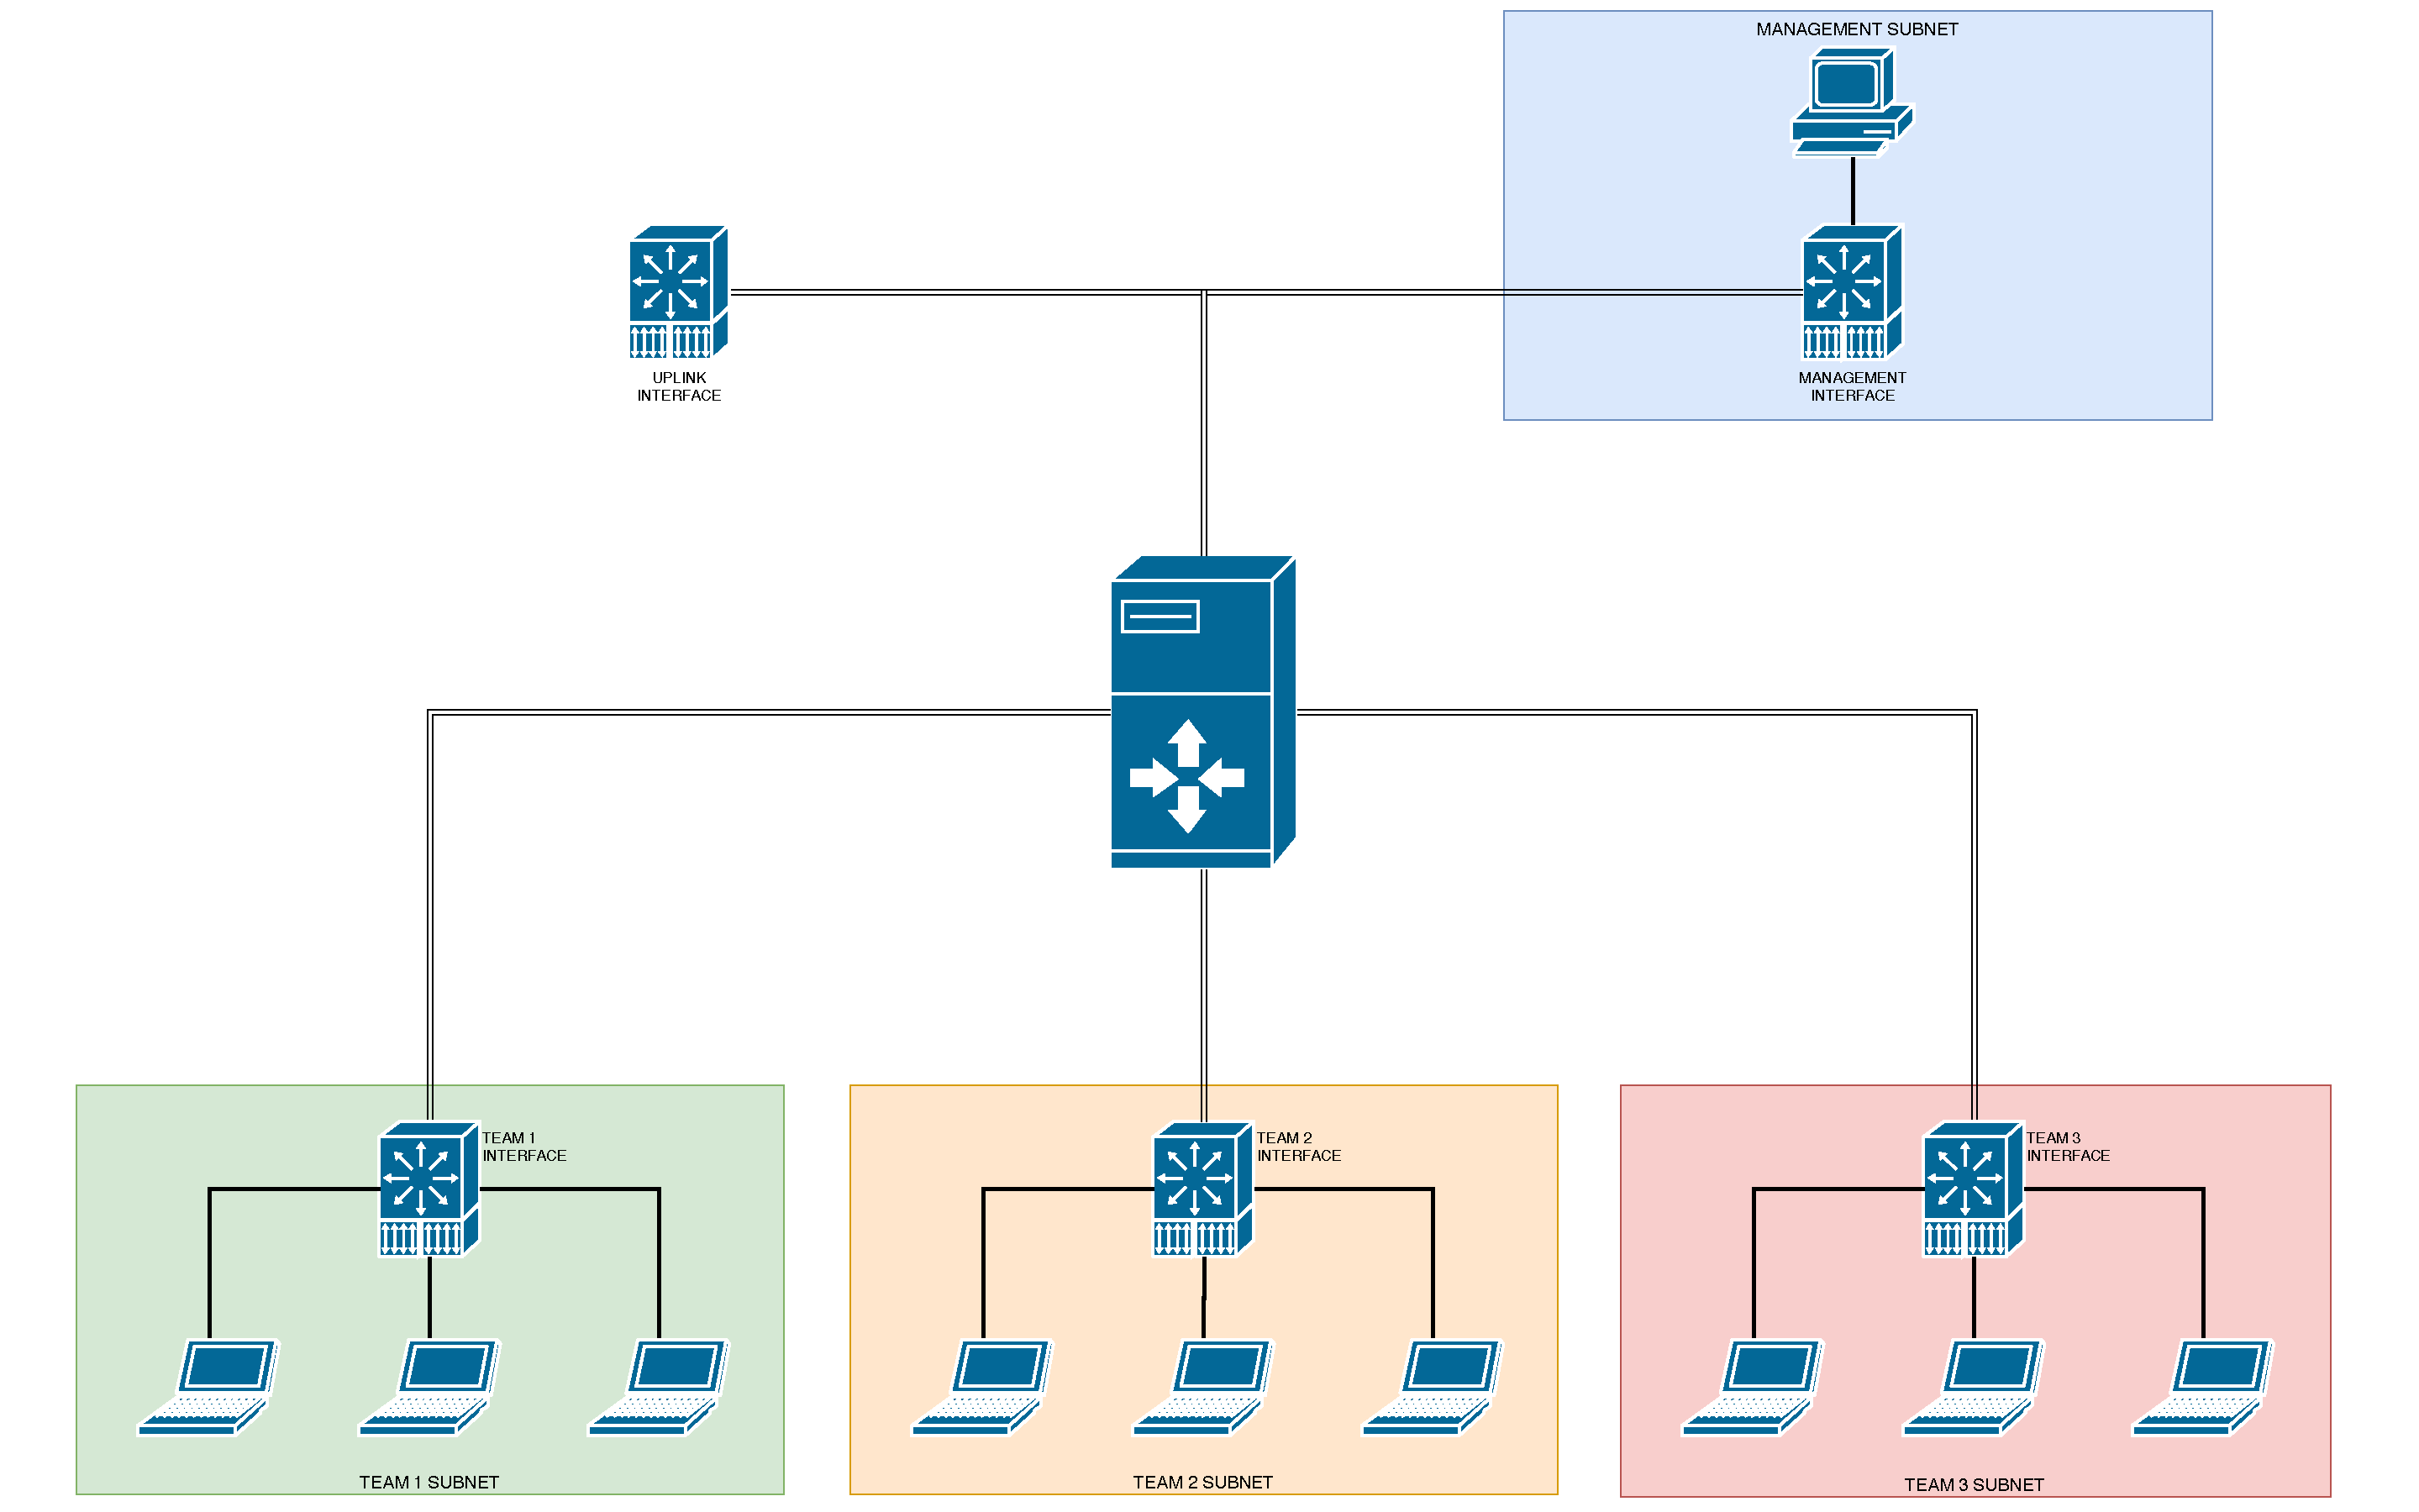
\includegraphics[width=\textwidth]{competition.pdf}

\end{frame}

\section{Tools \& Software}
\begin{frame}
    \frametitle{Software}
    \begin{itemize}
        \item <1-> iptables
        \item <2-> netplan
        \item <3-> script python
        \item <4-> script bash
    \end{itemize}
\end{frame}


\subsection*{iptables}
\begin{frame}
    \frametitle{Definizione}

    Iptables è un potente firewall integrato nel kernel Linux.
    Permette di definire, tramite regole, il filtraggio, la manipolazione dei pacchetti ed il NAT.
    \\~\\
    È strutturato in \textbf{tabelle}, ognuna contiene le proprie \textbf{catene} che possono, anche, essere definite dall'utente.
    \\~\\
    Ogni catena è una \textit{lista di regole} che specificano l'\textbf{azione} da intraprendere con i pacchetti che corrispondono alla regola.
    \\~\\
    Quest'\textit{azione} corrisponde al \textbf{target}.

\end{frame}

\begin{frame}
    \frametitle{TARGETS}

    Una regola di firewall specifica il criterio di selezione dei pacchetti ed il \textbf{target}.
    \\~\\
    \onslide<2-> {Se il pacchetto \textbf{non corrisponde} $\rightarrow$ verrà esaminata la \textbf{regola successiva}.}\\
    \onslide<3-> {Se il pacchetto \textbf{corrisponde} $\rightarrow$ verrà intrapresa l'azione definita dal \textit{target}}\onslide<4->{, che può essere:}
    \begin{description}
        \item[ACCEPT] <4-> lascia transitare il pacchetto
        \item[DROP] <5-> scarta il pacchetto
        \item[RETURN] <6-> ferma la "traversata" dell'attuale catena e ritorna alla catena chiamante (precedente)
        \item[catena definita dall'utente] <7->
    \end{description}
\end{frame}


\begin{frame}
    \frametitle{CHAINS}
    Le catene predefinite sono:
    \begin{description}
        \item[INPUT]<1-> per i pacchetti destinati ad un processo del server locale
        \item[OUTPUT]<2-> per i pacchetti creati dal server locale
        \item[FORWARD]<3-> per i pacchetti inoltrati tramite il server locale
        \item[POSTROUTING]<4-> per l'alterazione dei pacchetti appena prima dell'uscita
        \item[PREROUTING]<5-> per l'alterazione dei pacchetti appena entrati
    \end{description}
\end{frame}


\begin{frame}
    \frametitle{TABLES}
    Ogni tabella ha le proprie catene:
    \begin{description}
        \item[filter]<1-> INPUT, FORWARD, OUTPUT.
        \item[nat]<2-> PREROUTING, INPUT, OUTPUT, POSTROUTING.
        \item[mangle]<3-> PREROUTING, INPUT, OUTPUT, POSTROUTING, FORWARD.
        \item[raw]<4-> PREROUTING, OUTPUT
        \item[security]<5-> INPUT, OUTPUT, FORWARD.
    \end{description}
\end{frame}

\subsection*{netplan}

\begin{frame}
    \frametitle{Netplan}

    \onslide<1-> {Netplan è uno strumento per la configurazione del netwoking sui sistemi linux.}
    \\~\\
    \onslide<2-> {Sfrutta un file di configurazione in formato YAML (Yet Another Markup Language)} \onslide<3->{con:}
    \begin{itemize}
        \item <3-> le interfacce da utlizzare
        \item <4-> i parametri di configurazione per ogni interfaccia
        \item <5-> il \textbf{renderer} da utilizzare.
    \end{itemize}
    % \\~\\
    \onslide<6-> {Da questo file, Netplan, genera la configurazione finale per il \textit{renderer} scelto.}
\end{frame}

\begin{frame}
    \frametitle{Configurazione netplan}
    Supponiamo di avere tre TEAM e le seguenti interfacce:
    \begin{description}
        \item [ens33] interfaccia di UPLINK
        \item [ens37]<2-> interfaccia per il subnet di MANAGEMENT
        \item [ens38]<3-> interfaccia per il subnet del TEAM 1 
        \item [ens39]<4-> interfaccia per il subnet del TEAM 2
        \item [ens40]<5-> interfaccia per il subnet del TEAM 3
    \end{description}
    % Inoltre, supponiamo di volere un indirizzo IP
\end{frame}

\begin{frame}[fragile]
    \frametitle{Configurazione netplan}
    Con le interfacce definite prima avremo:
    \begin{lstlisting}
    network:
        ethernets:
            ens33:
                dhcp4: true
                dhcp6: false
            ens37:
                addresses:
                - 172.168.2.128/24
                dhcp4: false
                dhcp6: false
            ens38:
                addresses:
                - 172.168.3.100/24
                dhcp4: false
                dhcp6: false
    \end{lstlisting}
\end{frame}

\begin{frame}[fragile]
    \frametitle{Configurazione netplan}
    \begin{lstlisting}
            ens39:
                addresses:
                - 172.168.4.100/24
                dhcp4: false
                dhcp6: false
            ens40:
                addresses:
                - 172.168.5.100/24
                dhcp4: false
                dhcp6: false
        renderer: networkd
        version: 2
    \end{lstlisting}
\end{frame}


\subsection*{script python}
\begin{frame}
    \frametitle{Script realizzato in python}

    Lo script esegue tutto il lavoro di configurazione, sia per netplan sia per le regole di firewall (quindi iptables).
    \\~\\
    Per essere eseguito, lo script, ha bisogno di alcuni parametri in input.
    \\~\\
    Esso genera un file di configurazione, in formato JSON, editabile anche manualmente, che viene utilizzato per configurare la competizione.

\end{frame}

\begin{frame}[fragile]
    \frametitle{Formato file di configurazione}
    \begin{lstlisting}
        "ManagementInterface": "ens37",
        "ManagementInterfaceAddress": "172.168.2.100",
        "NumberOfTeams": 3,
        "Team1Interface": "ens38",
        "Team1InterfaceAddress": "172.168.3.100",
        "Team2Interface": "ens39",
        "Team2InterfaceAddress": "172.168.4.100",
        "Team3Interface": "ens40",
        "Team3InterfaceAddress": "172.168.5.100",
        "UplinkAddress": "172.168.1.128",
        "UplinkInterface": "ens33",
        "Log": "3/sec"
    \end{lstlisting}
\end{frame}


\begin{frame}
    \frametitle{Parametri dello script}
    \begin{description}
        \item[-I] configura la gara in modo interattivo
        \item[-G]<2-> mostra la configurazione attuale (del file di config)
        \item[-L]<3-> mostra tutte le interfacce della macchina
        \item[-p]<4-> per specificare la fase (1 o 2)
        \item[-ui]<5-> nome dell'interfaccia di uplink
        \item[-ua]<6-> indirizzo dell'interfaccia di uplink
        \item[-mi]<7-> nome dell'interfaccia di Management
        \item[-ma]<8-> indirizzo dell'interfaccia di Management
        \item[-masq]<9-> come effettuare il masquerading (false, IP singolo, IP per ogni squadra, true)
        \item[-t]<10-> le interfacce delle squadre
        \item[-l]<11-> il limite di logging
    \end{description}
\end{frame}

\section{Regole Firewall}
\subsection{Fase 1}
\subsubsection{Obiettivi}
\begin{frame}
    \frametitle{Obiettivi Fase 1}
    \begin{itemize}
        \item<1-> Isolamento dei Team
        \item<2-> Solo Management e Virtual Router possono iniziare una connessione verso gli altri
        \item<3-> Solo Management e Virtual Router possono connettersi all'esterno, attraverso l'UPLINK
        \item<4-> LOG dei pacchetti entranti e dei pacchetti inoltrati
    \end{itemize}

\end{frame}

\lstset{style=bash}
\subsubsection{Regole specifiche per il Virtual Router}
\begin{frame}[fragile]
    \frametitle{Regole specifiche per il Virtual Router}
    Connessione all'esterno attraverso UPLINK
    \\~\\
    \begin{lstlisting}[language=sh]
        $ iptables -P OUTPUT ACCEPT

        
        $ iptables -P INPUT DROP
        

        $ iptables -A INPUT -m conntrack --ctstate ESTABLISHED -j ACCEPT           
    \end{lstlisting}
\end{frame}

\begin{frame}[fragile]
    \frametitle{Regole specifiche per il Virtual Router}
    Ricevere connessioni da MANAGEMENT (qualsiasi tipo)
    \\~\\
    \begin{lstlisting}[language=sh]
        $ iptables -P INPUT DROP
        
        
        $ iptables -A INPUT -i $MANAGEMENT_INTERFACE -j ACCEPT
        
        
        $ iptables -P OUTPUT ACCEPT           
    \end{lstlisting}
\end{frame}

\begin{frame}[fragile]
    \frametitle{Regole specifiche per il Virtual Router}
    Connessioni ai TEAM e ricezione risposta
    \\~\\
    \begin{lstlisting}[language=sh]
        $ iptables -P OUTPUT ACCEPT
        
        
        $ iptables -A INPUT -m conntrack --ctstate ESTABLISHED -j ACCEPT           
    \end{lstlisting}
\end{frame}

\begin{frame}[fragile]
    \frametitle{Regole specifiche per il Virtual Router}
    Connessione loopback
    \\~\\
    \begin{lstlisting}[language=sh]
        $ iptables -P OUTPUT ACCEPT


        $ iptables -A INPUT -i lo -j ACCEPT           
    \end{lstlisting}
\end{frame}

\begin{frame}[fragile]
    \frametitle{Regole specifiche per il Virtual Router}
    Blocco connessioni dall'esterno e dai TEAM (se non iniziate da VR)
    \\~\\
    \begin{lstlisting}[language=sh]
        $ iptables -P INPUT DROP


        $ iptables -A INPUT -m conntrack --ctstate ESTABLISHED -j ACCEPT
    \end{lstlisting}
\end{frame}


\subsubsection{Regole specifiche per il Management}
\begin{frame}[fragile]
    \frametitle{Regole specifiche per il Management}
    Connessione all'esterno attraverso UPLINK
    \\~\\
    \begin{lstlisting}
        $ iptables -P FORWARD DROP

        
        $ iptables -t nat -A POSTROUTING -o $UPLINK -j MASQUERADE
        
        
        $ iptables -A FORWARD -i $MANAGEMENT_INTERFACE -j ACCEPT
        
        
        $ iptables -A FORWARD -m conntrack --ctstate ESTABLISHED -j ACCEPT
    \end{lstlisting}
\end{frame}

\begin{frame}[fragile]
    \frametitle{Regole specifiche per il Management}
    Connessione al VIRTUAL ROUTER
    \\~\\
    \begin{lstlisting}
        $ iptables -P INPUT DROP
        
        
        $ iptables -A INPUT -i $MANAGEMENT_INTERFACE -j ACCEPT
        
        
        $ iptables -P OUTPUT ACCEPT

    \end{lstlisting}
\end{frame}

\begin{frame}[fragile]
    \frametitle{Regole specifiche per il Management}
    Connessione ai TEAM
    \\~\\
    \begin{lstlisting}
        $ iptables -P FORWARD DROP
        
        
        $ iptables -A FORWARD -i $MANAGEMENT_INTERFACE -j ACCEPT
        
        
        $ iptables -A FORWARD -m conntrack --ctstate ESTABLISHED -j ACCEPT
    \end{lstlisting}
\end{frame}

\begin{frame}[fragile]
    \frametitle{Regole specifiche per il Management}
    Blocco connessioni dall'esterno e dai TEAM (se non iniziate da MANAGEMENT)
    \\~\\
    \begin{lstlisting}[language=sh]
        $ iptables -P INPUT DROP


        $ iptables -A INPUT -m conntrack --ctstate ESTABLISHED -j ACCEPT
    \end{lstlisting}
\end{frame}

\subsubsection{Regole specifiche per i Team}
\begin{frame}[fragile]
    \frametitle{Regole specifiche per i Team}
    Rispondere a connessioni iniziate da MANAGEMENT
    \\~\\
    \begin{lstlisting}
        $ iptables -P FORWARD DROP
        
        
        $ iptables -A FORWARD -m conntrack --ctstate ESTABLISHED -j ACCEPT
    \end{lstlisting}

\end{frame}
\begin{frame}[fragile]
    \frametitle{Regole specifiche per i Team}
    Rispondere a connessioni iniziate da VR
    \\~\\
    \begin{lstlisting}
        $ iptables -P INPUT DROP
        
        
        $ iptables -A INPUT -m conntrack --ctstate ESTABLISHED -j ACCEPT
    \end{lstlisting}

\end{frame}

\begin{frame}[fragile]
    \frametitle{Regole specifiche per i Team}
    Blocco inizio connessioni verso:
    \begin{itemize}
        \item MANAGEMENT
            \begin{lstlisting}
        $ iptables -P FORWARD DROP
            \end{lstlisting}
        \item VIRTUAL ROUTER
            \begin{lstlisting}
        $ iptables -P INPUT DROP  
            \end{lstlisting}
        \item altri TEAM
            \begin{lstlisting}
        $ iptables -P FORWARD DROP
            \end{lstlisting}
        \item esterno tramite UPLINK
            \begin{lstlisting}
        $ iptables -P FORWARD DROP
            \end{lstlisting}
    \end{itemize}
\end{frame}

\begin{frame}[fragile]
    \frametitle{Regole per il LOG}
    LOG dei pacchetti entranti
    \\~\\
    \begin{lstlisting}
    $ iptables -N LOGGING
    
    
    $ iptables -A INPUT -j LOGGING
    
    
    $ iptables -A LOGGING -m limit --limit $LOGLIMIT -j LOG --log-prefix 
            "COMPETITION-LOG: " --log-level 4

    \end{lstlisting}

\end{frame}


\begin{frame}[fragile]
    \frametitle{Regole per il LOG}
    LOG dei pacchetti inoltrati
    \\~\\
    \begin{lstlisting}
    $ iptables -N LOGGING


    $ iptables -A LOGGING -m limit --limit $LOGLIMIT -j LOG --log-prefix 
            "COMPETITION-LOG: " --log-level 4
    
    
    $ iptables -A FORWARD -j LOGGING
    \end{lstlisting}

\end{frame}

\subsection{Fase 2}
\subsubsection{Obiettivi}
\begin{frame}
    \frametitle{Obiettivi Fase 2}
    \begin{itemize}
        \item<1-> Solo Management e Virtual Router possono iniziare una connessione verso chiunque
        \item<2-> Solo Management e Virtual Router possono connettersi all'esterno, attraverso l'UPLINK
        \item<3-> Team possono comunicare tra loro
        \item<4-> Team non possono iniziare connessioni verso MANAGEMENT e VIRTUAL ROUTER
        \item<4-> LOG dei pacchetti entranti e dei pacchetti inoltrati
    \end{itemize}
    

\end{frame}
\subsubsection{Regole specifiche per il Virtual Router}
\begin{frame}[fragile]
    \frametitle{Regole specifiche per il Virtual Router}
    Le regole rimangono le stesse della FASE 1
\end{frame}


\subsubsection{Regole specifiche per il Management}
\begin{frame}[fragile]
    \frametitle{Regole specifiche per il Management}
    Connessione all'esterno attraverso UPLINK
    \\~\\
    \begin{lstlisting}
        $ iptables -P FORWARD ACCEPT
    \end{lstlisting}
\end{frame}

\begin{frame}[fragile]
    \frametitle{Regole specifiche per il Management}
    Connessione al VIRTUAL ROUTER
    \\~\\
    \begin{lstlisting}
        $ iptables -P INPUT DROP
        
        
        $ iptables -A INPUT -i $MANAGEMENT_INTERFACE -j ACCEPT
        
        
        $ iptables -P OUTPUT ACCEPT

    \end{lstlisting}
\end{frame}

\begin{frame}[fragile]
    \frametitle{Regole specifiche per il Management}
    Connessione ai TEAM
    \\~\\
    \begin{lstlisting}
        $ iptables -P FORWARD ACCEPT
        
        
        $ iptables -A FORWARD -m conntrack --ctstate ESTABLISHED -j ACCEPT
    \end{lstlisting}
\end{frame}

\begin{frame}[fragile]
    \frametitle{Regole specifiche per il Management}
    Blocco connessioni dall'esterno e dai TEAM (se non iniziate da MANAGEMENT)
    \\~\\
    \begin{lstlisting}[language=sh]
        $ iptables -P FORWARD ACCEPT 
        
        
        $ iptables -A FORWARD -m conntrack --ctstate ESTABLISHED -j ACCEPT
        
        
        $ iptables -A FORWARD -o $MANAGEMENT_INTERFACE -j DROP        
    \end{lstlisting}
\end{frame}

\subsubsection{Regole specifiche per i Team}
\begin{frame}[fragile]
    \frametitle{Regole specifiche per i Team}
    Rispondere a connessioni iniziate da MANAGEMENT
    \\~\\
    \begin{lstlisting}
        $ iptables -P FORWARD ACCEPT 
        
        
        $ iptables -A FORWARD -m conntrack --ctstate ESTABLISHED -j ACCEPT
        
        
        $ iptables -A FORWARD -o $MANAGEMENT_INTERFACE -j DROP
    \end{lstlisting}

\end{frame}
\begin{frame}[fragile]
    \frametitle{Regole specifiche per i Team}
    Rispondere a connessioni iniziate da VR
    \\~\\
    \begin{lstlisting}
        $ iptables -P INPUT DROP
        
        
        $ iptables -A INPUT -m conntrack --ctstate ESTABLISHED -j ACCEPT
    \end{lstlisting}

\end{frame}

\begin{frame}[fragile]
    \frametitle{Regole specifiche per i Team}
    Connessioni verso altri TEAM
    \\~\\
    \begin{lstlisting}
        $ iptables -P FORWARD ACCEPT
    \end{lstlisting}

\end{frame}

\begin{frame}[fragile]
    \frametitle{Regole specifiche per i Team}
    Blocco inizio connessioni verso:
    \begin{itemize}
        \item MANAGEMENT
            \begin{lstlisting}
        $ iptables -P FORWARD ACCEPT


        $ iptables -A FORWARD -o $MANAGEMENT_INTERFACE -j DROP
            \end{lstlisting}
        \item VIRTUAL ROUTER
            \begin{lstlisting}
        $ iptables -P INPUT DROP  
            \end{lstlisting}
        \item esterno tramite UPLINK
            \begin{lstlisting}
        $ iptables -P FORWARD ACCEPT


        $ iptables -A FORWARD -o $UPLINK -j DROP
            \end{lstlisting}
    \end{itemize}
\end{frame}

\begin{frame}
    \frametitle{Regole per il LOG}
    Le regole sono le stesse della FASE 1
\end{frame}

\begin{frame}
    \frametitle{NAT}
    \onslide<1-> {Il NAT, ovvero \textit{Network Address Translation}, conosciuto anche come \textbf{network masquerading}, è una tecnica
    che consiste nel modificare gli \textbf{indirizzi IP} contenuti negli \textbf{header} dei pacchetti in transito su
    un sistema che agisce da \textbf{router} all'interno di una comunicazione tra due o più \textit{host}.}
    \\~\\
    \onslide<2-> {Nel nostro caso verrà mascherato l'indirizzo sorgente del pacchetto.}

\end{frame}

\begin{frame}
    \frametitle{MASQUERADING}
    Lo script è stato ideato per permettere quattro situazioni di \textit{masquerading}:
    \begin{itemize}
        \item <1-> Un indirizzo unico per tutti i TEAM\onslide <2->{, che può essere:}
        \begin{itemize}
            \item<2-> definito dall'amministratore di gara
            \item<3-> generato in modo casuale
        \end{itemize}
        \item<4-> Indirizzi diversi per tutti i TEAM\onslide <5->{, che possono essere:}
        \begin{itemize}
            \item <5-> definiti dall'amministratore di gara
            \item <6-> generati in modo casuale
        \end{itemize}
    \end{itemize}
\end{frame}

\begin{frame}[fragile]
    \frametitle{Regole per il Masquerading}

    La regola per il \textbf{masquerading} è strutturata in questo modo:
    \\~\\
    \begin{lstlisting}
    $ iptables -t nat -A POSTROUTING -o $interface -j SNAT 
            --to-source $MASQUERADING_ADDRESS
    \end{lstlisting}
\end{frame}

\section{Python Script}

\begin{frame}
    \frametitle{Ricordiamo i parametri accettati dallo script}
    \begin{description}
        \item[-I] configura la gara in modo interattivo
        \item[-G] mostra la configurazione attuale (del file di config)
        \item[-L] mostra tutte le interfacce della macchina
        \item[-p] per specificare la fase (1 o 2)
        \item[-ui] nome dell'interfaccia di uplink
        \item[-ua] indirizzo dell'interfaccia di uplink
        \item[-mi] nome dell'interfaccia di Management
        \item[-ma] indirizzo dell'interfaccia di Management
        \item[-masq] come effettuare il masquerading (false, IP singolo, IP per ogni squadra, true)
        \item[-t] le interfacce delle squadre
        \item[-l] il limite di logging
    \end{description}
\end{frame}

\begin{frame}[fragile]
    \frametitle{Esempi}
    \begin{lstlisting}
-p 1 -ui ens33 -mi ens37 -ma 172.168.2.100 -masq true -t ens38 ens39 ens40 -l 4/sec
    \end{lstlisting}
    Avrà i seguenti effetti sulla tabella FILTER:
    \begin{lstlisting}
Chain INPUT (policy DROP)
target     prot opt source               destination         
LOGGING    all  --  anywhere             anywhere            
ACCEPT     all  --  anywhere             anywhere            
ACCEPT     all  --  172.168.1.1          anywhere            
ACCEPT     all  --  anywhere             anywhere             ctstate ESTABLISHED
ACCEPT     all  --  anywhere             anywhere            

Chain FORWARD (policy DROP)
target     prot opt source               destination         
LOGGING    all  --  anywhere             anywhere            
ACCEPT     all  --  anywhere             anywhere            
ACCEPT     all  --  anywhere             anywhere             ctstate ESTABLISHED

Chain OUTPUT (policy ACCEPT)
target     prot opt source               destination         

Chain LOGGING (2 references)
target     prot opt source               destination         
LOG        all  --  anywhere             anywhere             limit: avg 4/sec 
                            burst 5 LOG level warning prefix "COMPETITION-LOG: "
    \end{lstlisting}
\end{frame}

\begin{frame}[fragile]
    \frametitle{Esempi}
    \begin{lstlisting}
-p 1 -ui ens33 -mi ens37 -ma 172.168.2.100 -masq true -t ens38 ens39 ens40 -l 4/sec
    \end{lstlisting}
    Avrà i seguenti effetti sulla tabella NAT:
    \begin{lstlisting}
Chain PREROUTING (policy ACCEPT)
target     prot opt source               destination         

Chain INPUT (policy ACCEPT)
target     prot opt source               destination         

Chain OUTPUT (policy ACCEPT)
target     prot opt source               destination         

Chain POSTROUTING (policy ACCEPT)
target     prot opt source               destination         
MASQUERADE  all  --  anywhere             anywhere 
    \end{lstlisting}
\end{frame}

\begin{frame}[fragile]
    \frametitle{Esempi}
    \begin{lstlisting}
-p 1 -ui ens33 -mi ens37 -ma 172.168.2.100 -masq true -t ens38 ens39 ens40 -l 4/sec
            \end{lstlisting}
    Avrà i seguenti effetti sulla configurazione delle interfacce:
    \begin{lstlisting}
ens33: flags=4163<UP,BROADCAST,RUNNING,MULTICAST>  mtu 1500
        inet 172.168.1.128  netmask 255.255.255.0  broadcast 172.168.1.255

ens37: flags=4163<UP,BROADCAST,RUNNING,MULTICAST>  mtu 1500
        inet 172.168.2.100  netmask 255.255.255.0  broadcast 172.168.2.255

ens38: flags=4163<UP,BROADCAST,RUNNING,MULTICAST>  mtu 1500
        inet 172.168.3.100  netmask 255.255.255.0  broadcast 172.168.3.255

ens39: flags=4163<UP,BROADCAST,RUNNING,MULTICAST>  mtu 1500
        inet 172.168.4.100  netmask 255.255.255.0  broadcast 172.168.4.255

ens40: flags=4163<UP,BROADCAST,RUNNING,MULTICAST>  mtu 1500
        inet 172.168.5.100  netmask 255.255.255.0  broadcast 172.168.5.255

lo: flags=73<UP,LOOPBACK,RUNNING>  mtu 65536
        inet 127.0.0.1  netmask 255.0.0.0
    \end{lstlisting}
\end{frame}

\begin{frame}[fragile]
    \frametitle{Esempi}
    \begin{lstlisting}
-p 2 -ui ens33 -mi ens37 -ma 172.168.2.100 -masq true -t ens38 ens39 ens40 -l 4/sec
    \end{lstlisting}
    Avrà i seguenti effetti sulla tabella FILTER:
    \begin{lstlisting}
Chain INPUT (policy DROP)
target     prot opt source               destination         
LOGGING    all  --  anywhere             anywhere            
ACCEPT     all  --  anywhere             anywhere            
ACCEPT     all  --  172.168.1.1          anywhere            
ACCEPT     all  --  anywhere             anywhere             ctstate ESTABLISHED
ACCEPT     all  --  anywhere             anywhere            

Chain FORWARD (policy ACCEPT)
target     prot opt source               destination         
LOGGING    all  --  anywhere             anywhere            
ACCEPT     all  --  anywhere             anywhere            
ACCEPT     all  --  anywhere             anywhere             ctstate ESTABLISHED
DROP       all  --  anywhere             anywhere            
DROP       all  --  anywhere             anywhere            

Chain OUTPUT (policy ACCEPT)
target     prot opt source               destination         

Chain LOGGING (2 references)
target     prot opt source               destination         
LOG        all  --  anywhere             anywhere             limit: avg 4/sec 
                            burst 5 LOG level warning prefix "COMPETITION-LOG: "
    \end{lstlisting}
\end{frame}

\begin{frame}[fragile]
    \frametitle{Esempi}
    \begin{lstlisting}
-p 2 -ui ens33 -mi ens37 -ma 172.168.2.100 -masq true -t ens38 ens39 ens40 -l 4/sec
    \end{lstlisting}
    Avrà i seguenti effetti sulla tabella NAT:
    \begin{lstlisting}
Chain PREROUTING (policy ACCEPT)
target     prot opt source               destination         

Chain INPUT (policy ACCEPT)
target     prot opt source               destination         

Chain OUTPUT (policy ACCEPT)
target     prot opt source               destination         

Chain POSTROUTING (policy ACCEPT)
target     prot opt source               destination         
MASQUERADE  all  --  anywhere             anywhere            
SNAT        all  --  anywhere             anywhere             to:136.133.12.28
SNAT        all  --  anywhere             anywhere             to:76.138.130.11
SNAT        all  --  anywhere             anywhere             to:11.49.228.130
    \end{lstlisting}
\end{frame}

\begin{frame}[fragile]
    \frametitle{Esempi}
    \begin{lstlisting}
-p 1 -ui ens33 -mi ens37 -ma 172.168.2.100 -masq true -t ens38 ens39 ens40 -l 4/sec
            \end{lstlisting}
    Avrà i seguenti effetti sulla configurazione delle interfacce:
    \begin{lstlisting}
ens33: flags=4163<UP,BROADCAST,RUNNING,MULTICAST>  mtu 1500
        inet 172.168.1.128  netmask 255.255.255.0  broadcast 172.168.1.255

ens37: flags=4163<UP,BROADCAST,RUNNING,MULTICAST>  mtu 1500
        inet 172.168.2.100  netmask 255.255.255.0  broadcast 172.168.2.255

ens38: flags=4163<UP,BROADCAST,RUNNING,MULTICAST>  mtu 1500
        inet 172.168.3.100  netmask 255.255.255.0  broadcast 172.168.3.255

ens39: flags=4163<UP,BROADCAST,RUNNING,MULTICAST>  mtu 1500
        inet 172.168.4.100  netmask 255.255.255.0  broadcast 172.168.4.255

ens40: flags=4163<UP,BROADCAST,RUNNING,MULTICAST>  mtu 1500
        inet 172.168.5.100  netmask 255.255.255.0  broadcast 172.168.5.255

lo: flags=73<UP,LOOPBACK,RUNNING>  mtu 65536
        inet 127.0.0.1  netmask 255.0.0.0
    \end{lstlisting}
\end{frame}


\begin{frame}[fragile]
    \frametitle{Esempi}
    \begin{lstlisting}
-p 2 -ui ens33 -mi ens37 -ma 172.168.2.100 -masq 123.123.123.123
                                            -t ens38 ens39 -l 4/sec
    \end{lstlisting}
    Avrà i seguenti effetti sulla tabella FILTER:
    \begin{lstlisting}
Chain INPUT (policy DROP)
target     prot opt source               destination         
LOGGING    all  --  anywhere             anywhere            
ACCEPT     all  --  anywhere             anywhere            
ACCEPT     all  --  172.168.1.1          anywhere            
ACCEPT     all  --  anywhere             anywhere             ctstate ESTABLISHED
ACCEPT     all  --  anywhere             anywhere            

Chain FORWARD (policy ACCEPT)
target     prot opt source               destination         
LOGGING    all  --  anywhere             anywhere            
ACCEPT     all  --  anywhere             anywhere            
ACCEPT     all  --  anywhere             anywhere             ctstate ESTABLISHED
DROP       all  --  anywhere             anywhere            
DROP       all  --  anywhere             anywhere            

Chain OUTPUT (policy ACCEPT)
target     prot opt source               destination         

Chain LOGGING (2 references)
target     prot opt source               destination         
LOG        all  --  anywhere             anywhere             limit: avg 4/sec 
                            burst 5 LOG level warning prefix "COMPETITION-LOG: "
    \end{lstlisting}
\end{frame}

\begin{frame}[fragile]
    \frametitle{Esempi}
    \begin{lstlisting}
-p 2 -ui ens33 -mi ens37 -ma 172.168.2.100 -masq 123.123.123.123
                                            -t ens38 ens39 -l 4/sec

    \end{lstlisting}
    Avrà i seguenti effetti sulla tabella NAT:
    \begin{lstlisting}
Chain PREROUTING (policy ACCEPT)
target     prot opt source               destination         

Chain INPUT (policy ACCEPT)
target     prot opt source               destination         

Chain OUTPUT (policy ACCEPT)
target     prot opt source               destination         

Chain POSTROUTING (policy ACCEPT)
target     prot opt source               destination         
MASQUERADE  all  --  anywhere             anywhere            
SNAT        all  --  anywhere             anywhere             to:123.123.123.123
SNAT        all  --  anywhere             anywhere             to:123.123.123.123
    \end{lstlisting}
\end{frame}

\begin{frame}[fragile]
    \frametitle{Esempi}
    \begin{lstlisting}
-p 2 -ui ens33 -mi ens37 -ma 172.168.2.100 -masq 123.123.123.123 
                                            -t ens38 ens39 -l 4/sec

            \end{lstlisting}
    Avrà i seguenti effetti sulla configurazione delle interfacce:
    \begin{lstlisting}
ens33: flags=4163<UP,BROADCAST,RUNNING,MULTICAST>  mtu 1500
        inet 172.168.1.128  netmask 255.255.255.0  broadcast 172.168.1.255

ens37: flags=4163<UP,BROADCAST,RUNNING,MULTICAST>  mtu 1500
        inet 172.168.2.100  netmask 255.255.255.0  broadcast 172.168.2.255

ens38: flags=4163<UP,BROADCAST,RUNNING,MULTICAST>  mtu 1500
        inet 172.168.3.100  netmask 255.255.255.0  broadcast 172.168.3.255

ens39: flags=4163<UP,BROADCAST,RUNNING,MULTICAST>  mtu 1500
        inet 172.168.4.100  netmask 255.255.255.0  broadcast 172.168.4.255

lo: flags=73<UP,LOOPBACK,RUNNING>  mtu 65536
        inet 127.0.0.1  netmask 255.0.0.0
    \end{lstlisting}
\end{frame}

% \section{Test delle prestazioni}
% \begin{frame}
%     \frametitle{}

    

% \end{frame}


\end{document}


